\section{Results}
\label{sec:results}

\subsection{Synthetic Evaluation}

We evaluate three illustrative variants on the same fixed toy split. The
values are invented for this fixture, but the presentation follows the shape
of an ordinary experimental section: a metric table, a curve, and a visual
diagnostic. The important browser behaviors are captions, labels, references,
and readable figures rather than the numerical ranking.

\begin{figure}[t]
  \centering
  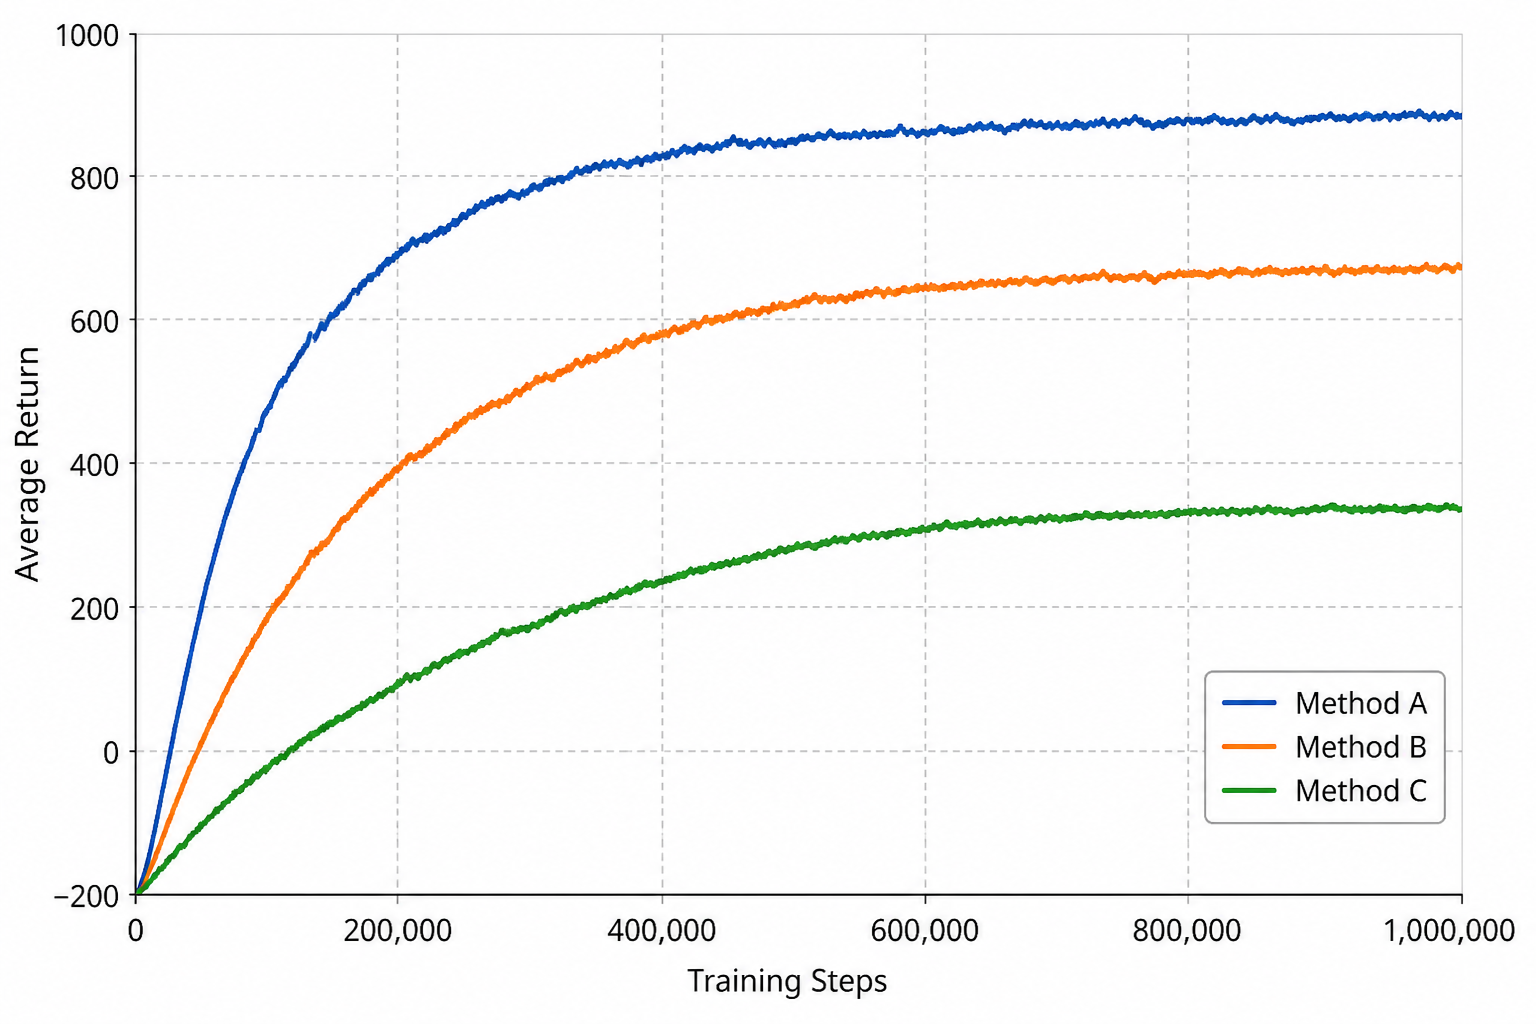
\includegraphics[width=0.94\linewidth]{figures/learning_curves.png}
  \caption{Synthetic training curves for three variants.}
  \label{fig:curves}
\end{figure}

As shown in Figure~\ref{fig:curves}, the variants have different trajectories
even though their final scores are close. A human reviewer should be able to
select the caption or surrounding explanation and attach feedback to it.

\begin{table}[t]
  \centering
  \caption{Synthetic evaluation results.}
  \label{tab:results}
  \begin{tabular}{lrrrr}
    \toprule
    Variant & Accuracy & Calibration & Parameters & Steps \\
    \midrule
    Baseline & 0.81 & 0.73 & 12.4k & 1000 \\
    Residual & 0.87 & 0.82 & 18.1k & 1000 \\
    Attention & 0.89 & 0.85 & 21.7k & 1200 \\
    \bottomrule
  \end{tabular}
\end{table}

Table~\ref{tab:results} is compact, while the wide table in the previous
section deliberately tests horizontal overflow. Both should remain readable
in the semantic HTML projection.

\subsection{A Visual Diagnostic}

The final diagnostic is a small attention-like matrix. It is not copied from
any published work; it only provides a structured image with repeated cells,
axes, and a caption for renderer testing.
\begin{figure}[t]
  \centering
  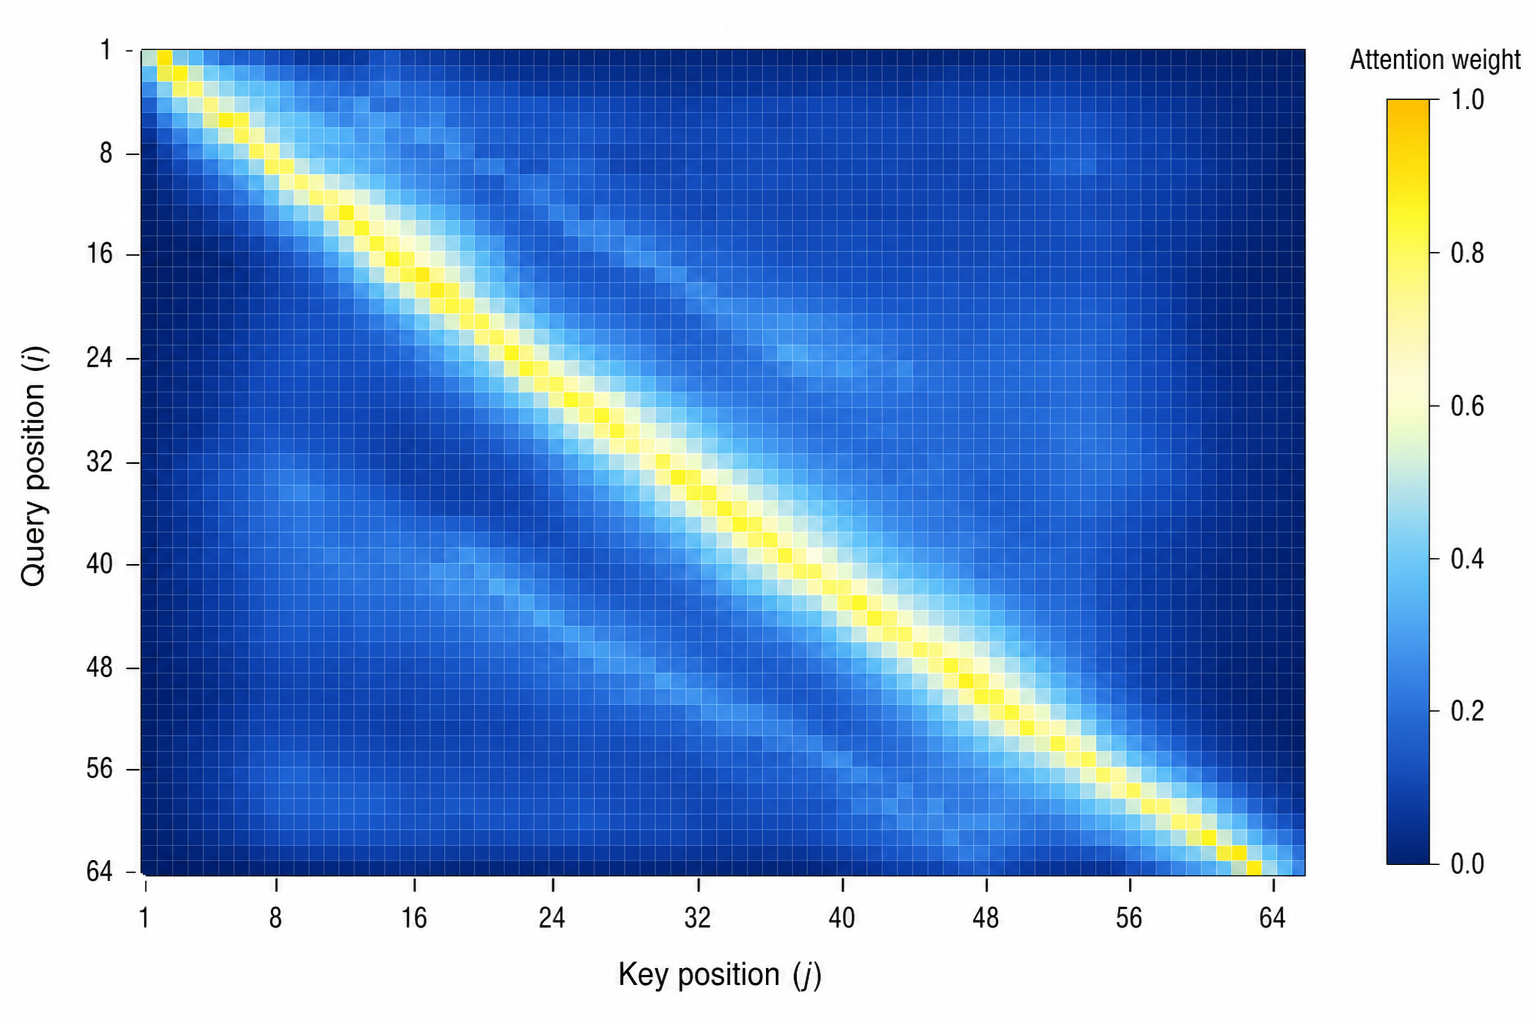
\includegraphics[width=0.66\linewidth]{figures/attention_map.png}
  \caption{Synthetic token-to-token interaction matrix.}
  \label{fig:attention}
\end{figure}
